\documentclass[10pt, uplatex, dvipdfmx]{jsarticle}
\usepackage{../mypackage}

\graphicspath{{../pictures}}

\setcounter{section}{6}

\begin{document}

\section{2重積分とは}

$2$ 変数関数の積分を定義する.

\subsection{2変数関数の Riemann 和}

$f$ を以下の有界な長方形 $K$ で定義された有界な $2$ 変数関数とする.
\[
  K=[a,b] \times [c,d] :=\Set{(x,y) | a \leq x \leq b, \, c \leq y \leq d}
\]

区間 $[a,b]$ を $m$ 個に,区間 $[c,d]$ を $n$ 個に分割し,長方
形 $K$ を $mn$ 個に分割する.
\begin{align*}
  & a=x_0 < x_1 < x_2 < \cdots < x_{m-1} < x_{m}=b\\
  & c=y_0 < y_1 < y_2 < \cdots < y_{n-1} < y_{n} =d
\end{align*}
この $(m+n+2)$ 個の点の組
$\Delta=\left( x_0, \ldots, x_n; y_0, \ldots,
  y_n\right)$ を $K$ の\textbf{分割}と呼ぶ.各小長方形から代表
点
$\left( \xi_{ij}, \eta_{ij}\right) \in [x_{i-1}, x_{i}] \times
[y_{j-1}, y_{j}]$ を選ぶ.このとき,
\[
  R\left( \Delta, \Set{(\xi_{ij}, \eta_{ij})}, f\right) 
  := \sum_{i=1}^{m} \sum_{j=1}^{n} f\left( \xi_{ij}, \eta_{ij}\right)(x_{i}-x_{i-1})(y_{j}-y_{j-1})
\]
を分割 $\Delta$ と代表点集合 $\Set{(\xi_{ij}, \eta_{ij})}$ に関す
る $f$ の\textbf{Riemann 和}という.

ここで定義した Riemann 和は下図のように,底面積
が $(x_{i}-x_{i-1})(y_{j}-y_{j-1})$ で,高さが
$f\left( \xi_{ij}, \eta_{ij}\right)$ の細長い直方体たちの体積を足し合わ
せたものである.これは $z=f(x,y)$ のグラフと $xy$ 平面と平
面 $x=a, \ x=b, \ y=c, \ y=d$ で囲まれた図形の体積を近似してい
る.ただし,グラフが $xy$ 平面より下にある部分の Riemann 和は負の値である.
\begin{figure}[h]
  \centering
  \includegraphics[height=8.5cm]{07/box.pdf}
\end{figure}

\newpage

簡単な Riemann 和を実際に計算してみよう.

\begin{example}
  $\ds f(x,y) = x^2+y^2$
  とする.下図のように,$\Delta=\left(x_0, x_1, x_2; y_0, y_1, y_2\right) = \left(0,
    \frac{1}{2}, 1;\ 0, \frac{1}{2}, 1\right)$
  を正方形$[0,1] \times [0,1]$の分割とし,各小長方形
  $[x_{i-1}, x_{i}] \times [y_{j-1}, y_j]$ の中心を $(\xi_{ij},
  \eta_{ij})$ とする.
  \begin{figure}[h]
    \centering
    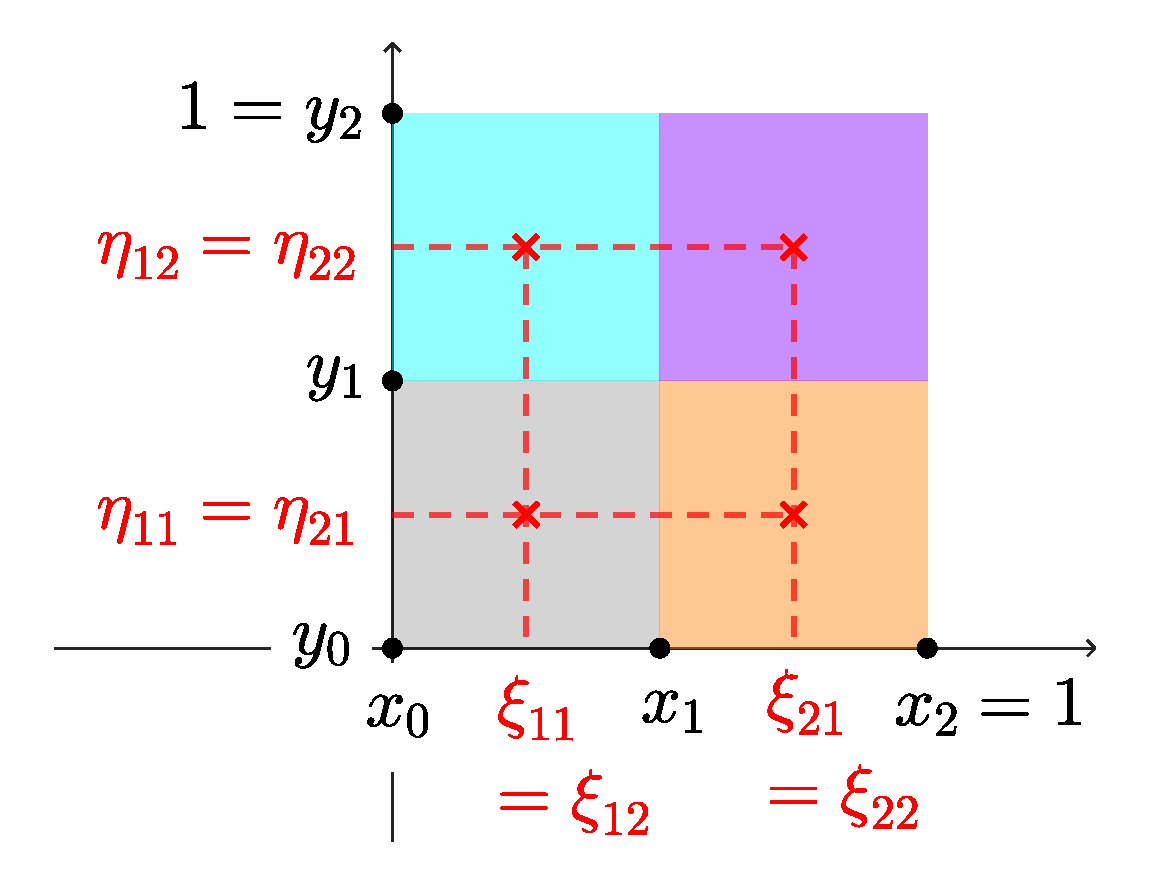
\includegraphics[height=5cm]{07/Rep3D.pdf}\\
  \end{figure}
  
  \noindent 代表点たちの具体的な座標は以下の通りである.
  \[
    \left( \xi_{11}, \eta_{11}\right) = \left( \frac{1}{4},
      \frac{1}{4}\right), \quad \left( \xi_{12}, \eta_{12}\right) =
    \left( \frac{1}{4}, \frac{3}{4}\right), \quad \left(\xi_{21},
      \eta_{21}\right) = \left(\frac{3}{4}, \frac{1}{4}\right), \quad
    \left( \xi_{22}, \eta_{22}\right) = \left( \frac{3}{4},
      \frac{3}{4}\right)
  \]
  この分割 $\Delta$と代表点集合 $\Set{\left( \xi_{ij}, \eta_{ij}
    \right)}$ に関する関数 $f(x,y)$ の Riemann 和は
  \[
    \begin{aligned}
      R\left( \Delta, \Set{(\xi_{ij}, \eta_{ij})}, f\right)
      =& \sum_{i=i}^{2} \sum_{j=1}^{2} f( \xi_{ij}, \eta_{ij}) (x_{i} - x_{i-1}) (y_{j} - y_{j-1})\\[2ex]
       =& f(\xi_{11}, \eta_{11})(x_1-x_0)(y_1-y_0) + f(\xi_{12}, \eta_{12}) (x_1-x_0)(y_2-y_1)\\[1ex]
       &+ f(\xi_{21}, \eta_{21})(x_2-x_1)(y_1-y_0)+ f(\xi_{22}, \eta_{22})(x_2-x_1)(y_2-y_1)\\[2ex]
      =& f\left(\frac{1}{4}, \frac{1}{4}\right)\left(\frac{1}{2}-0\right)\left(\frac{1}{2}-0\right)
         + f\left(\frac{1}{4}, \frac{3}{4}\right)\left(\frac{1}{2}-0\right)\left(1-\frac{1}{2}\right)\\
       &+ f\left(\frac{3}{4}, \frac{1}{4}\right)\left(1-\frac{1}{2}\right)\left(\frac{1}{2}-0\right)
         + f\left(\frac{3}{4}, \frac{3}{4}\right)\left(1-\frac{1}{2}\right)\left(1-\frac{1}{2}\right)\\[1ex]
      &= \frac{1}{32} + \frac{5}{32} + \frac{5}{32} + \frac{9}{32} = \frac{5}{8}
    \end{aligned}
  \]
  である.この値は下図の4個の直方体の体積の和に等しい.
  \begin{figure}[h]
    \centering
    \includegraphics[height=4.5cm]{07/boxes3D.png}                                                
  \end{figure}
  
\end{example}

\newpage

\subsection{ 2重積分の定義}

$f$ を有界な長方形 $K=[a,b] \times [c,d]$ で有界な $2$ 変数関数とする.
長方形 $K$ の分割
\[
  \Delta=\left( x_0, \ldots, x_m; \ y_0, \ldots, y_n\right)
\]
に対し,
\[
  |\Delta| := \max_{1 \leq i \leq m, \ 1 \leq j \leq n} \Set{ (x_{i}-x_{i-1}), \ (y_{j}-y_{j-1})}
\]
とする.$|\Delta| \to 0$ のとき,分割の仕方と代表点集
合 $\Set{(\xi_{ij}, \eta_{ij})}$ の取り方によらず Riemann
和$R\left( \Delta, \Set{(\xi_{ij}, \eta_{ij})}, f\right)$ が一定の値に
収束するならば,$f$ は $K$ で\textbf{(Riemann) 重積分
  可能} であるという.このとき,その極限値を以下のように表し,$f$ の $K$ 上の\textbf{$2$ 重積分}という.
\begin{equation}\label{eq:double-int}
  \iint_{K} f(x,y) \ dx dy
\end{equation}

$2$ 変数関数が重積分可能であるかどうかを調べるのは $1$ 変数関数のとき以
上に難しいが,$1$ 変数関数のときと同様に,有界な長方形 $[a,b] \times
[c,d]$ 上の連続関数は重積分可能であることが知られている.


\begin{theorem}\label{thm:double-integrable}
  有界な長方形 $K=[a,b] \times [c,d]$ 上連続な $2$ 変数関数は $K$ で重積分可能である.
\end{theorem}

$2$ 変数関数 $f$ が有界な長方形 $K=[a,b] \times [c,d]$ で連続であれ
ば,$K$ のいかなる分割 $\Delta$ と代表点集合に対しても,$|\Delta| \to
0$ でさえあれば必ず Riemann 和は一定の値に近づき,その値
が(\ref{eq:double-int})に等しいことをこの定理\ref{thm:double-integrable}は主張
している.\\



より一般の有界閉領域 $D$ に対しては,下図のように $D$ を含む長方形 $K=[a,b] \times
[c,d]$ を1つ取り,
\[
  f^{*}(x,y) =\left\{
    \begin{array}{cc}
      f(x,y) & \left( (x,y) \in D\right)\\
      0 & \left( (x,y) \not\in D\right)
    \end{array}
  \right.
\]
として,$f^{*}$ が $K$ 上重積分可能なら $f$ は $D$ 上重積分可能であるとし,
\[
  \iint_{D} f(x,y) \ dx dy = \iint_{K}f^{*}(x,y) \ dx dy
\]
によって $f$ の $D$ 上の2重積分を定義する.$D$ 上の重積分の値
は $D$ を含む長方形 $K$ の取り方によらない.
\begin{figure}[h]
  \centering
  \includegraphics[height=5cm]{07/region.pdf}
\end{figure}


\newpage

\subsection{2重積分の諸性質}

\begin{theorem}[$2$ 重積分の線形性]
  $f, g$ を有界閉領域 $D$ 上重積分可能な $2$ 変数関数とする.定
  数 $\alpha, \beta \in \mathbb{R}$ に対して以下が成り立つ.
  \[
    \iint_{D}\left( \alpha f(x,y) + \beta g(x,y)\right) dx dy 
    =\alpha \iint_{D} f(x,y) \ dx dy + \beta \iint_{D} f(x,y) \ dx dy
  \]
\end{theorem}

\begin{theorem}
  $2$ つの有界閉領域 $D_1, D_2$ の共通部分 $D_1 \cap D_2$ の面積が $0$
  のとき,$D_1 \cup D_2$ 上重積分可能な関数 $f$ に対して以下が成り立つ.
  \[
    \iint_{D_1 \cup D_2} f(x,y) \ dx dy = \iint_{D_1} f(x,y) \ dx dy + \iint_{D_2} f(x,y) \ dx dy
  \]
  \begin{table}[h]
    \centering
    \begin{tabular}{|cc|c|}\hline
      \multicolumn{2}{|c|}{$D_1 \cap D_2$ の面積 $=0$} & $D_1 \cap D_2$ の面積 $>0$\\ \hline
      \includegraphics[height=3cm]{07/disjoint.pdf}
     &\includegraphics[height=3cm]{07/tangent.pdf}
     & \includegraphics[height=3cm]{07/intersect.pdf}\\ \hline
    \end{tabular}
  \end{table}
\end{theorem}

\begin{theorem}\label{thm:additiveD}
  $2$ 変数関数 $f,g$ が有界閉領域 $D$ 上重積分可能かつ $f(x,y) \geqq g(x,y)$ なら以下が成り立つ.
  \[
    \iint_{D} f(x,y) \ dx dy \geqq \iint_{D} g(x,y) \ dx dy
  \]
  \begin{figure}[h]
    \centering
    \includegraphics[height=5cm]{07/monotonic.png}
  \end{figure}
\end{theorem}

\begin{theorem}
  有界閉領域 $D$ 上重積分可能な $2$ 変数関数 $f$ に対して以下が成り立つ.
  \[
    \left| \iint_{D} f(x,y) \ dx dy \right| \leqq \iint_{D} \left| f(x,y) \right| dx dy
  \]
\end{theorem}


\newpage

\subsection{累次積分による 2重積分の計算}

長方形上の連続関数の2重積分は累次積分によって
計算できる.

\begin{theorem}\label{thm:int-on-square}
  長方形 $[a,b] \times [c,d]$ 上の連続関数 $f$ に対して以下が成り立つ.
  \[
    \iint_{[a,b] \times [c,d]} f(x,y) \ dx dy = \int_{a}^{b} \left( \int_{c}^{d} f(x,y) \ dy \right) \ dx
    = \int_{c}^{d} \left( \int_{a}^{b} f(x,y) \ dx \right) \ dy
  \]
\end{theorem}

次節でこの定理\ref{thm:int-on-square}を拡張し,より一般的な有界閉領域上の2重積分の計算方法を与える.\\

\begin{example}
  \[
    \begin{aligned}
      \iint_{[0,1] \times [0,2]} \left( x^2+y^2\right) \ dx dy
      &= \int_{0}^{1} \left( \int_{0}^{2} (x^2+y^2) \ dy \right) \ dx
        = \int_{0}^{1} \left[ x^2y + \frac{y^3}{3} \right]_{y=0}^{y=2} \ dx\\[1ex]
      & = \int_{0}^{1} \left( 2x^2 + \frac{8}{3}\right) \ dx = \left[\frac{2}{3}x^3 + \frac{8}{3}x \right]_{0}^{1}
        =\frac{10}{3}
    \end{aligned}
  \]
  あるいは,次のようにも計算できる.
  \[
    \begin{aligned}
        \iint_{[0,1] \times [0,2]} \left( x^2+y^2\right) \ dx dy
      &= \int_{0}^{2} \left( \int_{0}^{1} (x^2+y^2) \ dx \right) \ dy
        = \int_{0}^{2} \left[ \frac{x^3}{3} + xy^2 \right]_{x=0}^{x=1} \ dy\\
      & = \int_{0}^{2} \left( \frac{1}{3} + y^2\right) \ dy
        = \left[ \frac{y}{3} + \frac{y^3}{3}\right]_{0}^{2}=\frac{10}{3}
    \end{aligned}
  \]
\end{example}

\vspace{1zh}

\begin{example}
  \[
    \begin{aligned}
      \iint_{[0,\pi]\times [0, \pi/3]} \sin(x-y) \ dx dy
      &= \int_{0}^{\pi} \left( \int_{0}^{\pi/3} \sin (x-y) \ dy \right) \ dx
        = \int_{0}^{\pi} \Big[ \cos(x-y) \Big]_{y=0}^{y=\pi/3} \ dx \\[1ex]
      &= \int_{0}^{\pi} \left( \cos\left( x - \frac{\pi}{3}\right) - \cos x\right) \ dx
        = \left[ \sin\left( x - \frac{\pi}{3}\right) - \sin x\right]_{0}^{\pi}\\[1ex]
      &= \sin \frac{2\pi}{3} - \sin\left( -\frac{\pi}{3}\right) =  \sqrt{3}
    \end{aligned}
  \]
  あるいは,次のようにも計算できる.
  \[
    \begin{aligned}
      \iint_{[0,\pi] \times [0, \pi/3]} \sin(x-y) \ dx dy
      &= \int_{0}^{\pi/3} \left( \int_{0}^{\pi} \sin(x-y) \ dx \right) \ dy
        = \int_{0}^{\pi/3} \Big[ -\cos(x-y) \Big]_{x=0}^{x=\pi} \ dy\\
      &= \int_{0}^{\pi/3}\left( -\cos\left(\pi-y\right) + \cos\left(-y\right) \right) \ dy
        =\Big[ \sin(\pi-y) + \sin y\Big]_{0}^{\pi/3}\\[1ex]
      &= \sin\frac{2\pi}{3} + \sin\frac{\pi}{3} = \sqrt{3}
    \end{aligned}
  \]
\end{example}

\newpage

\subsection{練習問題}

次の長方形上の2重積分を計算しよう.

\vspace{1zh}

\begin{enumerate}[(1)]

  \setlength{\itemsep}{2zh}
  
\item $\ds \iint_{[-1,1] \times [1.2]} \left( x^3-y^2\right) \ dx dy$

\item $\ds \iint_{[0,1] \times [-1,0]} e^{2x-3y} \ dx dy$

\item $\ds \iint_{[0,2] \times [0,1]} x e^{xy} \ dx dy$

\item $\ds \iint_{\left[0, \pi/2\right] \times [1,e]} \left( \cos x \right) \log y \ dx dy$
\end{enumerate}

\begin{figure}[b]
答え : (1) $\ds -\frac{14}{3}$ \quad (2) $\ds \frac{1-e^2-e^3+e^5}{6}$ \quad (3) $\ds e^2-3$ \quad (4) $1$
\end{figure}

\newpage

\subsection{(おまけ)Riemann 和の極限としての2重積分}

\vspace{1zh}

長方形上の2重積分の値を Riemann 和の極限として計算する例を挙げておく.\\


\begin{example}
  $\ds \iint_{[0,1] \times [0,1]} \left( x^2+y^2\right) \ dx dy$

  \vspace{1zh}
  
  正方形 $[0,1]\times [0,1]$ を $x$ 方向と $y$ 方向それぞれ $n$ 等分し
  て得られる分割を
  \[
    \Delta_n = \left( x_0, x_1, \ldots, x_n \ ; \ y_0, y_1, \ldots,
      y_n\right)
  \]
  とし,各小正方形 $[x_{i-1}, x_{i}] \times [y_{j-1}, y_{j}]$ の中心(対角線の交点)を代
  表点 $\left( \xi_{ij}, \eta_{ij}\right)$ とする.つまり,
  \[
    x_i = \frac{i}{n}, \quad y_j = \frac{j}{n}, \quad \xi_{ij} =
    \frac{x_{i-1}+x_{i}}{2}, \quad \eta_{ij}=\frac{y_{j-1}+y_{j}}{2}
  \]
  である.この分割 $\Delta_n$と代表点集合 $\Set{\left( \xi_{ij},
      \eta_{ij}\right)}$ に関する $f(x,y) =
  x^2+y^2$ の Riemann 和を $S_n$ とする.
  \[
    S_n := R \left(\Delta_n, \Set{\left( \xi_{ij}, \eta_{ij}\right)}, f \right)
    = \sum_{i=1}^{n} \sum_{j=1}^{n} f\left( \xi_{ij}, \eta_{ij}\right) (x_i-x_{i-1})(y_{j}-y_{j-1})
  \]
  $f$ は $[0,1] \times [0,1]$ で連続なので,定理\ref{thm:double-integrable} か
  らこの $S_n$ は $n \to \infty$ のとき収束し,
  \[
      \lim_{n \to \infty} S_n = \iint_{[0,1] \times [0,1]} (x^2+y^2) \ dx dy
  \]
  である.各 $x_{i}-x_{i-1}, y_{j}- y_{j-1}$ はいずれも $\ds
  \frac{1}{n}$
  であり,$\ds \xi_{ij} = \frac{2i-1}{2n}, \; \eta_{ij} =
  \frac{2j-1}{2n}$ なので
  \[
    \begin{aligned}
      S_n &= \sum_{i=1}^{n} \sum_{j=1}^{n} \left(\left(\frac{2i-1}{2n}\right)^2
            + \left(\frac{2j-1}{2n}\right)^2\right) \cdot \frac{1}{n} \cdot \frac{1}{n}
            = \frac{1}{4n^4} \left( \sum_{i=1}^{n} \sum_{j=1}^{n} (2i-1)^2
            + \sum_{j=1}^{n} \sum_{i=1}^{n} (2j-1)^2\right)\\[1ex]
          &= \frac{1}{4n^4} \cdot 2 \sum_{i=1}^{n}\sum_{j=1}^{n} (2i-1)^2 = \frac{1}{2n^4} \sum_{i=1}^{n} n (2i-1)^2
            = \frac{1}{4n^4} \sum_{i=1}^{n} \left( 4i^2-4i+1\right)\\[1ex]
          &=\frac{1}{2n^3} \left( 4 \sum_{i=1}^{n} i^2 - 4 \sum_{i=1}^{n} + \sum_{i=1}^{n}1\right)
            = \frac{1}{2n^3} \left( 4 \cdot \frac{n(n+1)(2n+1)}{6} - 4 \cdot \frac{n(n+1)}{2} + n \right)\\[1ex]
          &= \frac{1}{3}\left(1+\frac{1}{n}\right)\left(2+\frac{1}{n}\right) - \frac{1}{n}\left(1+\frac{1}{n}\right)
            + \frac{1}{2n^2} \to \frac{2}{3} \; (n \to \infty)
    \end{aligned}
  \]
  である.以上から,$\ds \iint_{[0,1] \times [0,1]} (x^2+y^2) \ dx dy = \lim_{n \to \infty} S_n = \frac{2}{3}$ である.
\end{example}

\newpage

定数関数 $f(x,y) = C$ は連続関数だが,定理\ref{thm:double-integrable}に頼ることなく直接2重積分を計算できる.\\

\begin{example}
  $\ds \iint_{[a,b]\times [c,d]}C \ dx dy$

  \vspace{1zh}

  $\Delta=(x_0, \ldots, x_m \ ;\  y_0, \ldots, y_n)$ を長方形
  $[a,b] \times [c,d]$ の分割とし,各小長方形
  $[x_{i-1}, x_{i}] \times [y_{j-1}, y_{j}]$ の代表点
  $\left( \xi_{ij}, \eta_{ij}\right)$ を任意に選ぶ.これらに関す
  る $f(x,y) =C$ の Riemann 和は
  \[
    \begin{aligned}
      R(\Delta, \Set{(\xi_{ij}, \eta_{ij})}, f)
      &= \sum_{i=1}^{m} \sum_{j=1}^{n} f(\xi_{ij}, \eta_{ij}) (x_{i}-x_{i-1})(y_{j}-y_{j-1})\\
      &= C \left( \sum_{i=1}^{m} (x_{i}-x_{i-1}) \right) \left(\sum_{j=1}^{n} (y_{j}-y_{j-1})\right)
        = C \left( x_{m} - x_{0} \right) \left( y_{n} - y_{0}\right)\\[1ex]
      &= C(b-a)(d-c)
    \end{aligned}
  \]
  である.よって,分割の仕方と代表点の選び方によらず Riemann 和は一定な
  ので,特に,$|\Delta | \to 0$ における極限値もその一定の値に等しい.
  よって,以下を得る.
  \[
    \iint_{[a,b] \times [c,d]} C \ dx dy = \lim_{|\Delta|
      \to 0} R\left(\Delta, \Set{\left(\xi_{ij}, \eta_{ij}\right)}, f\right) =
    C(b-a)(d-c)
  \]
\end{example}




\end{document}
